\section{Verwandte Arbeiten}
\subsection{Zuordnung von Vorschriften zu Geschäftsprozessen}
% Sätze 1-4 abgesegnet am 27.10.2026, Sätze 5 bis 12 am 28.10.2026
% "am nächsten an dieser Arbeit" wandert ans Ende von 3.1
Sai et al.~\cite{sai2024} vergleichen vier Verfahren, mit denen sich für einen Geschäftsprozess die relevanten Absätze aus einer Sammlung von Rechtstexten bestimmen lassen.
Beim ersten Verfahren ordnen Fachleute die Absätze von Hand zu: in der Studie drei Mitarbeitende eines australischen Versicherers und zwei Prozessexperten aus dem Bankwesen.
Beim zweiten Verfahren bewerten viele Laien über die Online-Plattform Amazon Mechanical Turk gegen eine geringe Bezahlung, ob ein Absatz zu einem Prozessschritt passt.
Das dritte Verfahren übersetzt Prozessschritte und Rechtsabsätze in Zahlenvektoren, sogenannte Embeddings, und sortiert die Absätze danach, wie ähnlich ihr Inhalt dem Prozessschritt ist (Abbildung~\ref{fig:embedding_karte}).
Beim vierten Verfahren legt man dem Sprachmodell GPT-4 jeden Absatz einzeln zusammen mit der Prozessbeschreibung vor, und das Modell entscheidet, ob der Absatz relevant ist.
Untersucht werden zwei Fallstudien: die Schadensbearbeitung einer Reiseversicherung und die Kundenprüfung einer Bank (\enquote{Know Your Customer}).
Jede Fallstudie ist in drei Ebenen gegliedert.
Die oberste Ebene ist der Prozess als Ganzes.
Darunter liegen die Teilprozesse, in die sich der Prozess gliedert.
Die unterste Ebene bilden die einzelnen Arbeitsschritte, die sogenannten Tasks.
Für jeden Absatz wird auf jeder Ebene geprüft, ob er dort relevant ist.
\offen{Beispiel für die drei Ebenen; später Übergang auf die gesamte Arbeit (nicht nur das Bewerbungsverfahren)}
Die Auswahl der Fachleute dient als Maßstab, mit dem die anderen drei Verfahren verglichen werden.
Gemessen wird, welchen Anteil der relevanten Absätze ein Verfahren findet (\fb{trefferquote}, englisch \emph{Recall}) und welcher Anteil der gemeldeten Absätze tatsächlich relevant ist (\fb{genauigkeit}, englisch \emph{Precision}).
Trefferquote und Genauigkeit werden für jede der drei Ebenen getrennt berechnet.
\offen{HIER WEITER: Block 2 -- Ergebnisse von Sai et al.\ je Ebene (Tabelle 3.1), danach Bezug zu dieser Arbeit (\enquote{am nächsten}, Vergleichswert für H2). Vorher H2-Schwelle klären: 0,62 stammt von der Teilprozess-Ebene, Task-Ebene 0,69/0,77. Herkunft der drei Ebenen wird in Abschnitt 2.1 erklärt.}

\begin{figure}[H]
  \centering
  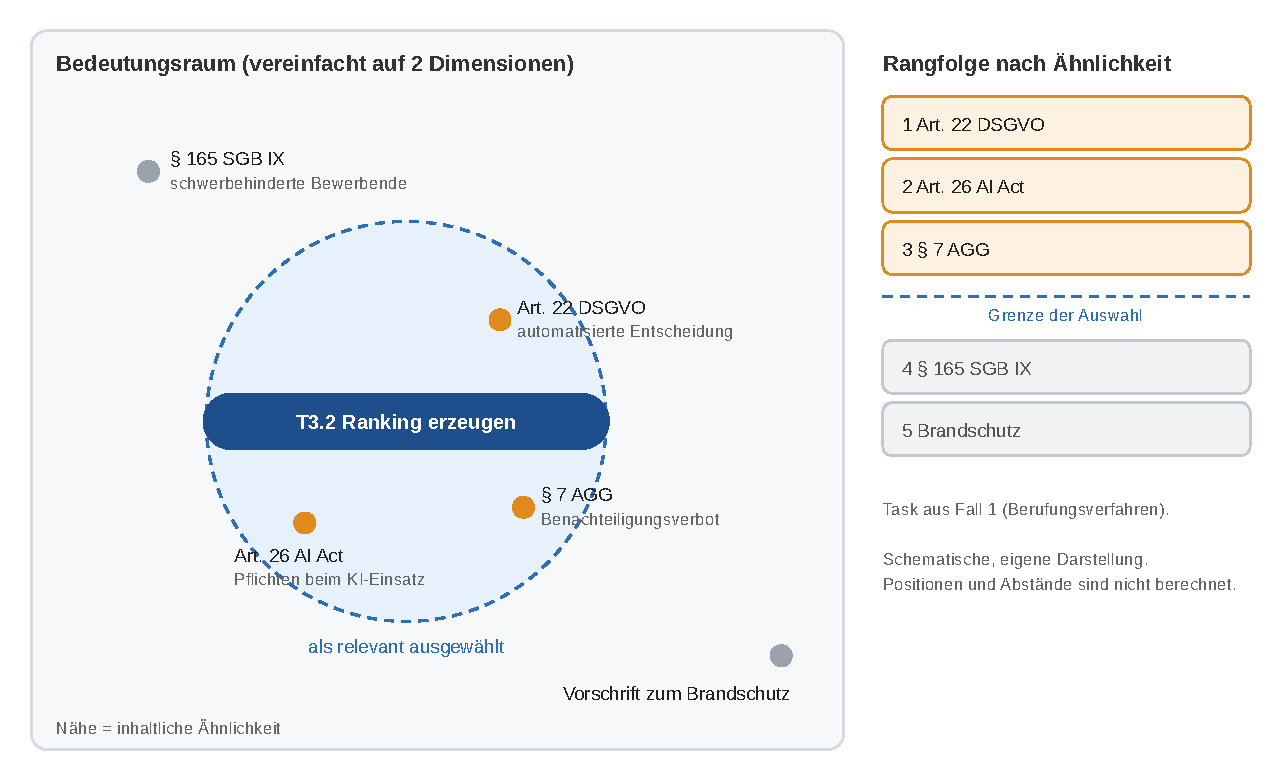
\includegraphics[width=\textwidth]{figures/abb_3_1_embedding_karte.pdf}
  \caption[Prinzip des Embedding-Verfahrens]{Prinzip des Embedding-Verfahrens am Beispiel dieser Arbeit. Je näher ein Rechtsabsatz am Prozessschritt liegt, desto ähnlicher ist sein Inhalt; ausgewählt werden die ähnlichsten Absätze. Schematische, eigene Darstellung; Positionen und Abstände sind nicht berechnet.}
  \label{fig:embedding_karte}
\end{figure}

\offen{weitere Sätze zu 3.1}

\subsection{Rechtsinformationssuche mit Sprachmodellen}
\offen{3.2 -- Literaturrecherche}

\subsection{Runtime Verification von Agenten}
% Sätze abgesegnet am 22.11.2026
Die Arbeit von Sai et al.~\cite{sai2024} endet mit der Zuordnung, also mit der Liste der Vorschriften, die für jeden Schritt des Prozesses gelten.
Diese Arbeit geht einen Schritt weiter und fragt, ob sich die zugeordneten Vorschriften auch während der Ausführung des Prozesses durchsetzen lassen (FF4).
Diese Frage wird wichtig, sobald ein KI-Agent Schritte des Prozesses selbst ausführt, etwa Bewerbungen auswertet oder Mails verschickt.
Dann muss jede Aktion des Agenten vor der Ausführung geprüft werden, damit er die Vorschriften einhält.
Solche Prüfungen heißen Runtime Verification (Laufzeitverifikation), weil sie das tatsächliche Verhalten eines Systems zur Laufzeit, also während der Ausführung, mit festgelegten Regeln vergleichen.
Kahani et al.~\cite{kahani2026} zeigen mit dem Verfahren C-Trace, dass sich dieser Ansatz auf KI-Agenten übertragen lässt, die mit Werkzeugen arbeiten.
C-Trace setzt dazu einen Monitor zwischen den Agenten und seine Werkzeuge.
Der Monitor zeichnet jeden Werkzeugaufruf auf, prüft vor der Ausführung, ob der Aufruf zusammen mit den bisherigen Aufrufen eine Regel verletzt, und blockiert ihn in diesem Fall.
Die Regeln bilden vier Grundsätze der DSGVO ab, etwa die Einwilligung vor der Verarbeitung und das Recht auf Löschung.
Hier liegt der Unterschied zu dieser Arbeit, denn Kahani et al. haben die vier Regeln von Hand geschrieben.
Sie setzen voraus, dass bekannt ist, welche Vorschriften für einen Prozess gelten und wie daraus Regeln entstehen.
Genau diese Schritte untersucht diese Arbeit, indem ein Agent die Vorschriften selbst findet und daraus die Regeln für den Monitor ableitet (H5 bis H7).
Damit verbindet die Arbeit die Zuordnung von Sai et al. mit der Durchsetzung von Kahani et al.
Für den Aufbau der eigenen Versuche dient C-Trace zusätzlich als methodisches Vorbild.
Kahani et al. prüfen den Monitor an vier Anwendungsfällen mit einem Sprachmodell (GPT-4o mini) als Agent.
Darunter sind ein medizinischer Assistent und die Kontoeröffnung bei einer Bank.
Der Agent ist bewusst so eingestellt, dass er jede Anfrage ausführt, damit allein der Monitor über die Zulässigkeit entscheidet.
Je Fall versuchen 400 Dialoge, den Agenten mit Mitteln wie Zeitdruck oder der Berufung auf eine Autorität zu einem Verstoß zu verleiten.
Dazu kommen harmlose Dialoge und harmlose Grenzfälle, die einem Verstoß ähneln, aber zulässig sind.
Gemessen wird, wie viele Angriffe trotz Monitor gelingen und wie viele harmlose Dialoge der Monitor fälschlich blockiert.
Mit Monitor liegt der Anteil gelungener Angriffe in allen vier Fällen bei 0\,\%, ebenso der Anteil der Fehlalarme.
Die Autoren weisen darauf hin, dass dieses Ergebnis nur gilt, wenn jeder Verstoß als Ereignis erfasst wird und eine Regel ihn abdeckt.
Genau diese Voraussetzung prüft diese Arbeit mit H7, denn dort stammen die Regeln aus den ungeprüften Ergebnissen des Agenten.

\subsection{Forschungslücke}
\offen{3.4}
